\documentclass[11pt,a4paper]{article}

% ===== Geometry & typography =====
\usepackage[a4paper, margin=25mm]{geometry}
\usepackage[T1]{fontenc}
\usepackage[utf8]{inputenc}
\usepackage{lmodern}
\usepackage[scaled=0.92]{helvet}
\usepackage{microtype}

% ===== Tables, math, figures =====
\usepackage{booktabs}
\usepackage{array}
\usepackage{tabularx}
\usepackage{colortbl}
\usepackage{xcolor}
\usepackage{graphicx}
\usepackage{caption}
\usepackage{subcaption}
\usepackage{amsmath, amssymb}
\usepackage{enumitem}
\usepackage{titlesec}
\usepackage{fancyhdr}
\usepackage{lastpage}
\usepackage{etoolbox}
\usepackage{xparse}
\usepackage{tcolorbox}
\tcbuselibrary{skins,breakable}
\usepackage{pgfgantt}

% ===== Bibliography =====
\usepackage[backend=biber, style=numeric, sorting=none]{biblatex}
\addbibresource{references.bib}

% ===== Brand colors =====
\definecolor{brandPrimary}{HTML}{C2410C}
\definecolor{brandSecondary}{HTML}{2563EB}
\definecolor{brandAccent}{HTML}{15803D}
\definecolor{brandAmber}{HTML}{B45309}
\definecolor{brandSlate}{HTML}{64748B}
\definecolor{rowAlt}{HTML}{F8FAFC}
\definecolor{nearBlack}{HTML}{1E293B}

% ===== Hyperref (load late) =====
\usepackage[colorlinks=true, linkcolor=brandSecondary, urlcolor=brandSecondary, citecolor=brandSecondary]{hyperref}
\usepackage[capitalise]{cleveref}

% ===== Section heading style =====
\titleformat{\section}
  {\sffamily\Large\bfseries\color{brandPrimary}}
  {\thesection}{0.6em}
  {}[\vspace{2pt}\hrule height 0.5pt]
\titleformat{\subsection}
  {\sffamily\large\bfseries\color{brandSecondary}}
  {\thesubsection}{0.5em}{}
\titleformat{\subsubsection}
  {\sffamily\normalsize\bfseries\color{nearBlack}}
  {\thesubsubsection}{0.4em}{}

% ===== Headers / footers =====
\pagestyle{fancy}
\fancyhf{}
\fancyhead[L]{\small\sffamily\color{brandSlate} SENG 474 \textbullet{} CineEmbed}
\fancyhead[R]{\small\sffamily\color{brandSlate} Intermediate Progress Report}
\fancyfoot[C]{\small\sffamily\color{brandSlate} Page \thepage{} of \pageref{LastPage}}
\renewcommand{\headrulewidth}{0.4pt}
\renewcommand{\footrulewidth}{0pt}

% ===== Custom commands =====
% \status{complete|inprogress|planned|deferred}
\newcommand{\status}[1]{%
  \ifstrequal{#1}{complete}{\colorbox{brandAccent}{\textcolor{white}{\sffamily\bfseries\small\,COMPLETE\,}}}{%
  \ifstrequal{#1}{inprogress}{\colorbox{brandAmber}{\textcolor{white}{\sffamily\bfseries\small\,IN PROGRESS\,}}}{%
  \ifstrequal{#1}{planned}{\colorbox{brandSecondary}{\textcolor{white}{\sffamily\bfseries\small\,PLANNED\,}}}{%
  \ifstrequal{#1}{deferred}{\colorbox{brandSlate}{\textcolor{white}{\sffamily\bfseries\small\,DEFERRED\,}}}{}}}}%
}

% Headline-number callout box
\newtcolorbox{headlinebox}{%
  colback=brandPrimary!8!white,
  colframe=brandPrimary,
  boxrule=0.6pt,
  arc=2pt,
  left=10pt, right=10pt, top=8pt, bottom=8pt,
}

% Risk callout box
\newtcolorbox{riskbox}[1]{%
  colback=brandAmber!6!white,
  colframe=brandAmber,
  boxrule=0.6pt,
  arc=2pt,
  title={#1},
  fonttitle=\sffamily\bfseries\small\color{white},
  coltitle=white,
  colbacktitle=brandAmber,
  left=8pt, right=8pt, top=6pt, bottom=6pt,
}

% Evidence prefix
\newcommand{\evidence}[1]{\textit{\color{brandSlate}\small Evidence: }\small #1}

% Big number on a line (used in headline boxes)
\newcommand{\bignumber}[1]{{\fontsize{36pt}{42pt}\sffamily\bfseries\color{brandPrimary}#1}}

% ===== Document =====
\begin{document}

% ----- Title page (no header/footer) -----
\thispagestyle{empty}
\vspace*{4cm}
\begin{center}
{\sffamily\Huge\bfseries\color{brandPrimary} CineEmbed} \\[0.4cm]
{\sffamily\Large Multi-Modal Unsupervised Embedding of 329{,}044 Films} \\[1.6cm]
{\sffamily\large\color{brandSecondary} Intermediate Progress Report \textbullet{} v1.0} \\[2.5cm]
{\large Ahmet Baran Dincoguz \quad\textbullet\quad Arda Arvas \quad\textbullet\quad Bertan Kaan Kaya} \\[1.0cm]
{\sffamily\normalsize SENG 474 --- Deep Learning, Spring 2026} \\
{\sffamily\normalsize TED University} \\[0.6cm]
{\sffamily\normalsize 2026-05-06} \\[1.5cm]
{\small\color{brandSlate}Repository: \href{https://github.com/bkaankaya/CineEmbed-A-Multi-Modal-Unsupervised-Film-Recommendation-System}{github.com/bkaankaya/CineEmbed-A-Multi-Modal-Unsupervised-Film-Recommendation-System}}
\end{center}
\vfill
\clearpage

% Body sections will be added in subsequent tasks.
% ===== Executive Summary =====
\section*{Executive Summary}
\addcontentsline{toc}{section}{Executive Summary}

\noindent\status{complete}\ \textbf{Modeling MVP phase delivered on schedule.} The intermediate phase of the CineEmbed project is on track: all three pre-registered hypotheses (H1, H2, H3) have been validated, six models have been trained and evaluated against three orthogonal label axes, and the deferred work for the final report has been scoped and prioritized.

\begin{itemize}[leftmargin=1.2em, itemsep=2pt, topsep=2pt]
  \item \textbf{Data engineering:} 564-dimensional feature matrix over 329{,}044 films, organized into seven block-contiguous modalities, frozen at v1.2.
  \item \textbf{Modeling:} six runs trained spanning three model tiers (non-deep baselines, simple deep, multi-modal deep + DEC fine-tune); evaluation completed against \texttt{primary\_genre}, \texttt{decade\_bin}, and \texttt{lang\_top10}.
  \item \textbf{Hypotheses:} H1 (DEC > AE on \texttt{genre\_NMI}), H2 (best-deep $\geq 1.10\times$ best-non-deep), H3 (NMI $> 0.15$ floor) all PASS; H2 by an order of magnitude.
\end{itemize}

\vspace{4pt}
\begin{headlinebox}
\noindent\bignumber{$+205\%$} \hfill \begin{minipage}[b]{0.65\linewidth}\raggedleft\small relative gain on \texttt{genre\_NMI} of the best deep model (\texttt{dec\_z64\_k21}: 0.332) over the strongest non-deep baseline (\texttt{kmeans\_raw\_k21}: 0.109). Pre-registered threshold for H2 was $+10\%$.\end{minipage}
\end{headlinebox}

\vspace{4pt}
\noindent\textbf{Hypothesis tracker:}

\begin{center}\small
\rowcolors{2}{rowAlt}{white}
\begin{tabularx}{\linewidth}{@{}l X r l@{}}
\toprule
\textbf{ID} & \textbf{Statement} & \textbf{Result} & \textbf{Status} \\
\midrule
H1 & DEC \texttt{genre\_NMI} > AE \texttt{genre\_NMI}              & $0.332 > 0.328$ & \status{complete} PASS \\
H2 & Best-deep \texttt{genre\_NMI} $\geq 1.10\times$ best-non-deep  & $+205\%$        & \status{complete} PASS \\
H3 & Best-deep \texttt{genre\_NMI} > 0.15 absolute floor            & $0.332 \gg 0.15$& \status{complete} PASS \\
\bottomrule
\end{tabularx}
\end{center}

\clearpage

% ===== 1. Project Overview =====
\section{Project Overview}
\label{sec:overview}

\subsection{Goal}
The CineEmbed project trains unsupervised 64-dimensional representations of movie metadata via multi-modal autoencoder and Deep Embedded Clustering (DEC) architectures, with the objective of demonstrating that the learned latent geometry recovers three orthogonal label axes --- primary genre, decade, and original language --- substantially better than non-deep KMeans baselines.

\subsection{Scope}
The dataset is a corpus of 329{,}044 films assembled from TMDB metadata, awards records (Oscar / BAFTA / Cannes), and Wikipedia-derived director biographies. The feature matrix has 564 dimensions organized into seven block-contiguous modalities:

\begin{center}\small
\rowcolors{2}{rowAlt}{white}
\begin{tabular}{@{}l r p{8.4cm}@{}}
\toprule
\textbf{Modality block} & \textbf{Dim} & \textbf{Contents} \\
\midrule
\texttt{numerical} & 6   & log\_popularity, log\_vote\_count, runtime\_norm, vote\_average\_norm, has\_vote, has\_engagement \\
\texttt{genre}     & 22  & 21-way one-hot + \texttt{has\_genre} flag \\
\texttt{language}  & 31  & top-30 original\_language one-hot + flag (sparse: $\sim$99\% zero per row) \\
\texttt{decade}    & 2   & decade\_norm + has\_release\_date \\
\texttt{awards}    & 6   & log-counts of prior Oscar / BAFTA / Cannes wins and nominations \\
\texttt{text}      & 384 & \texttt{all-MiniLM-L6-v2} sentence embeddings of overview + title \\
\texttt{director}  & 113 & bio\_pca\_64 + has\_director\_bio + dir\_lang\_30 + dir\_country\_18 + has\_director\_lang \\
\bottomrule
\end{tabular}
\end{center}

\noindent See \cref{fig:multilingual-coverage} for the long-tailed language distribution that motivates the language block's sparsity-aware treatment.

\begin{figure}[h]
\centering
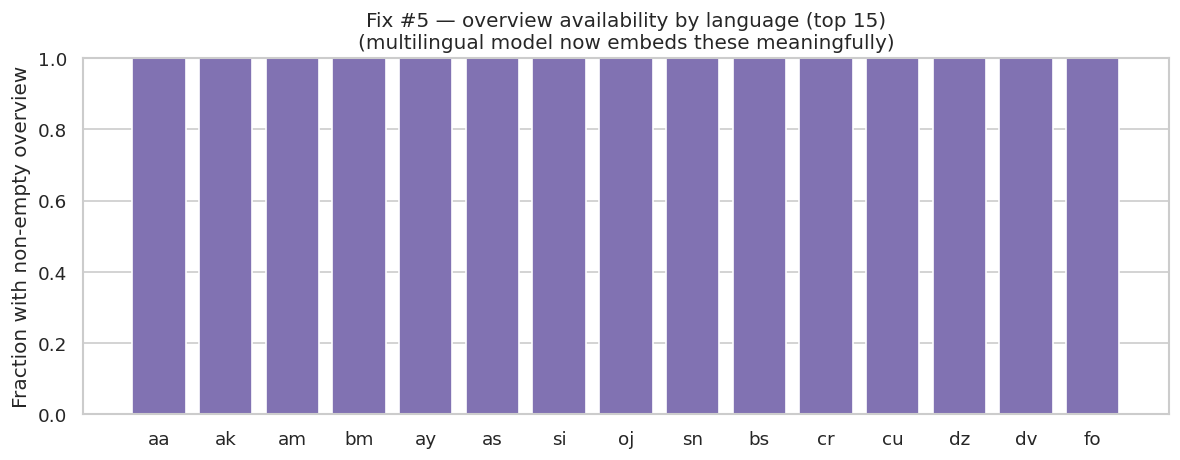
\includegraphics[width=0.78\linewidth]{../../artifacts/figures/multilingual_coverage.png}
\caption{Multilingual coverage of the 329{,}044-film corpus. Top-3 languages dominate; the long tail is what motivates the modality-specific projection design (\cref{sec:work-completed}).}
\label{fig:multilingual-coverage}
\end{figure}

\subsection{Team and Responsibilities}
\begin{center}\small
\rowcolors{2}{rowAlt}{white}
\begin{tabular}{@{}l p{10cm}@{}}
\toprule
\textbf{Member} & \textbf{Primary responsibility} \\
\midrule
Ahmet Baran Dincoguz & Architecture design, modeling pipeline, evaluation, repository ownership \\
Arda Arvas           & Data engineering, awards merge, feature blocks \\
Bertan Kaan Kaya     & Director-bio extension, UMAP analysis, presentation deliverables \\
\bottomrule
\end{tabular}
\end{center}

\clearpage

% ===== 2. Schedule & Milestones =====
\section{Schedule and Milestones}
\label{sec:schedule}

\subsection{Course Schedule (SENG 474, Spring 2026, Weeks 1--15)}

\noindent The project schedule is anchored to the SENG 474 syllabus, a 15-week semester running from 11/02 to 20/05. Course-mandated project deliverables fall on weeks W3 (team formation), W5 (proposal / abstract), W11 (intermediate report), and W14--W15 (project demo presentations). The Gantt chart below maps the project's internal phases against course weeks.

\begin{center}
\begin{ganttchart}[
  hgrid, vgrid,
  title height=1, title label font=\sffamily\small,
  bar height=0.55,
  bar/.append style={fill=brandSecondary, draw=brandSecondary},
  bar label font=\sffamily\small,
  group/.append style={fill=brandPrimary, draw=brandPrimary},
  group label font=\sffamily\bfseries\small\color{white},
  milestone/.append style={fill=brandAccent, draw=brandAccent},
  milestone label font=\sffamily\small,
  x unit=0.65cm,
  y unit chart=0.55cm,
]{1}{15}
  \gantttitle{SENG 474 Spring 2026 --- Week}{15} \\
  \gantttitlelist{1,...,15}{1} \\
  \ganttbar{Team \& proposal}{1}{5} \\
  \ganttmilestone{Proposal (W5)}{5} \\
  \ganttbar{Data engineering}{4}{7} \\
  \ganttbar{Architecture design}{6}{9} \\
  \ganttbar{Modeling MVP}{8}{11} \\
  \ganttmilestone{Intermediate report (W11)}{11} \\
  \ganttbar[bar/.append style={fill=brandAmber, draw=brandAmber}]{VAE family + ablations}{11}{14} \\
  \ganttbar[bar/.append style={fill=brandAmber, draw=brandAmber}]{Final report + demo prep}{13}{15} \\
  \ganttmilestone{Final demo (W14--15)}{15}
\end{ganttchart}
\end{center}

\subsection{Milestone Status}

\begin{center}\small
\rowcolors{2}{rowAlt}{white}
\begin{tabular}{@{}c l l l@{}}
\toprule
\textbf{Week} & \textbf{Date} & \textbf{Milestone} & \textbf{Status} \\
\midrule
W3   & 25/02     & Team formation submitted                  & \status{complete} \\
W5   & 11/03     & Project proposal / abstract               & \status{complete} \\
W7   & 25/03     & Midterm exam (course-wide)                & \status{complete} \\
W9--W11 & ---    & Six runs trained and evaluated            & \status{complete} \\
W11  & 22/04     & UMAP latent analysis                      & \status{complete} \\
W11  & 22/04     & \textbf{Intermediate Report Submission}   & \status{complete} \\
W12--W14 & ---   & VAE family + F1/F2/k-sweep ablations      & \status{planned} \\
W14  & 13/05     & Project demo (presentation 1)             & \status{planned} \\
W15  & 20/05     & Project demo (presentation 2)             & \status{planned} \\
W15  & 20/05     & Final Report + Demo Video                 & \status{planned} \\
\bottomrule
\end{tabular}
\end{center}

\clearpage

% ===== 3. Work Completed to Date =====
\section{Work Completed to Date}
\label{sec:work-completed}

\noindent Three phases have completed since project kickoff. Each subsection below summarizes the phase scope, the deliverables produced, and the empirical evidence supporting completion.

\subsection{Data engineering phase \hfill \status{complete}}
\label{sec:data-engineering}

\noindent The team assembled a unified feature matrix from three input sources:

\begin{itemize}[leftmargin=1.2em, itemsep=2pt, topsep=2pt]
\item \textbf{TMDB} --- 329{,}044 films, basic metadata (title, overview, runtime, language, genres, votes, popularity, release date).
\item \textbf{Awards records} --- Oscar, BAFTA, Cannes wins and nominations, merged on title and release year, used to compute prior log-counts as the \texttt{awards} block.
\item \textbf{Wikipedia director bios} --- raw text scraped per credited director, embedded with \texttt{all-MiniLM-L6-v2}~\cite{reimers2019sbert}, then projected to 64 components via PCA. Coverage is partial: 96.8\% of films lack a Wikipedia bio for any of their credited directors.
\end{itemize}

\noindent Three engineering decisions are worth noting because they shape the modeling phase:
\begin{enumerate}[leftmargin=1.4em, itemsep=2pt, topsep=2pt]
\item Sparse modalities (language, director-language, director-country) preserved as one-hot blocks rather than embedded, to keep them interpretable.
\item Missing release dates encoded as a binary flag (\texttt{has\_release\_date}) rather than imputed --- this turned out to be structurally relevant (see \cref{sec:modeling-mvp}).
\item Director-bio reconstruction loss masked by \texttt{has\_director\_bio} (G2 masking) so that 96.8\% of films contribute zero loss for that block, preventing the autoencoder from learning to predict zeros from zeros.
\end{enumerate}

\noindent\evidence{The frozen 564-dim feature matrix, EDA notebook (\texttt{notebooks/01\_eda.ipynb}), and 21 supporting figures under \texttt{artifacts/figures/}.}

\clearpage

\subsection{Architecture design phase \hfill \status{complete}}
\label{sec:architecture-design}

\noindent The team specified and implemented three model heads (deterministic AE, VAE, DEC) on a shared multi-modal backbone. The MVP uses AE and DEC; VAE is implemented but its training is deferred to the final report.

\subsubsection*{Multi-modal backbone}

The encoder applies seven independent \texttt{\_BlockProjection} layers, one per modality, each compressing its block to a fixed projection dimension before concatenation~\cite{gorishniy2021tabular}. The 164-dimensional concatenation feeds a shared backbone --- $\mathrm{Linear}(164{\to}128) \to \mathrm{ReLU} \to \mathrm{Dropout}(0.2) \to \mathrm{Linear}(128{\to}64)$ --- yielding the 64-dimensional latent $\mathbf{z}$. \cref{fig:architecture-multimodal} shows the schematic.

\begin{figure}[h]
\centering
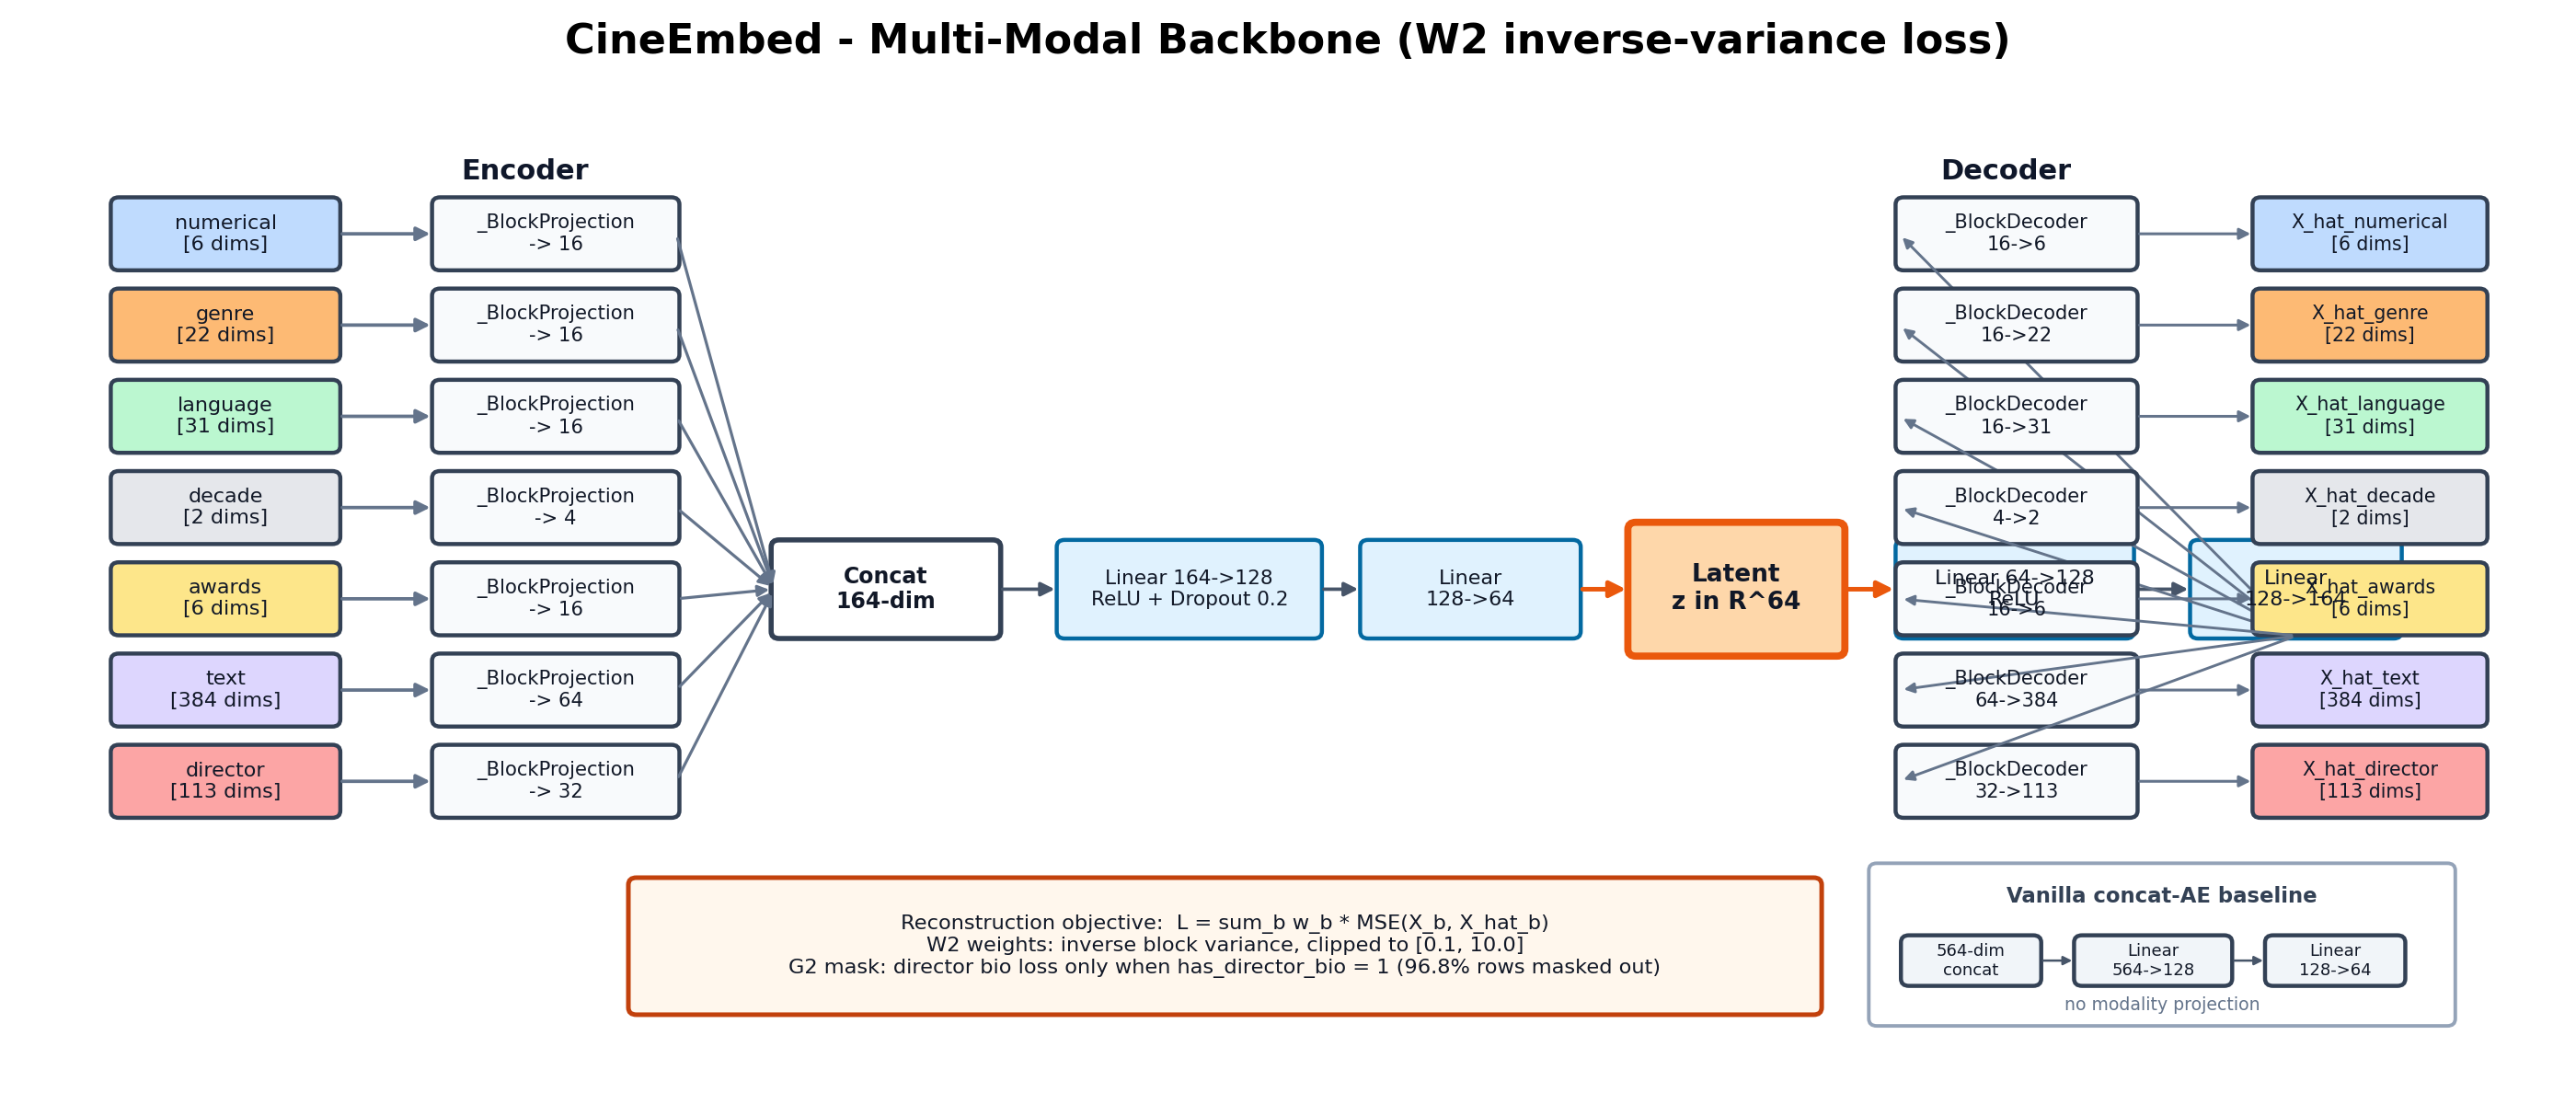
\includegraphics[width=0.95\linewidth]{../../figures/architecture_multimodal.png}
\caption{Multi-modal backbone. Seven modality-specific projection blocks reduce each feature group to its proj\_dim; the resulting 164-dim concatenation feeds a shared backbone with a 64-dim bottleneck. Decoder heads mirror the input structure.}
\label{fig:architecture-multimodal}
\end{figure}

\subsubsection*{Loss functions}

\noindent\textbf{W2 inverse-variance weighting (canonical).} Per-block reconstruction losses are reweighted by the inverse of each block's variance, with clipping for numerical stability:
\[
\mathcal{L}_{\mathrm{W2}} = \sum_{b=1}^{7} w_b \cdot \mathrm{MSE}(X_b, \hat{X}_b), \qquad w_b = \mathrm{clip}\!\left(\tfrac{1}{\mathrm{Var}(X_b)},\, 0.1,\, 10.0\right).
\]
The clip bounds $[0.1, 10.0]$ are a peer-review-driven safety measure that prevents the language block (with very low average variance) from dominating early training.

\noindent\textbf{W1 (ablation).} Uniform weights $w_b = 1$ for all blocks. Identical architecture and training schedule as W2. This run isolates the contribution of inverse-variance weighting from modality projection.

\noindent\textbf{G2 director-bio masking.} Element-wise multiplication of the \texttt{bio\_pca\_64} reconstruction loss by \texttt{has\_director\_bio} so that bio-less rows contribute zero loss for that sub-block.

\noindent\textbf{DEC fine-tuning.} Soft assignments $q_{ij} = (1 + \lVert z_i - \mu_j \rVert^2)^{-1}$ over $k=21$ centroids initialized via KMeans++ on pre-trained AE latents; auxiliary target $p_{ij} = q_{ij}^2 / \sum_i q_{ij}$ computed per batch (10$\times$ speedup over full-dataset target with no measurable quality regression)~\cite{xie2016dec,guo2017idec}. Total loss $\gamma \cdot \mathrm{KL}(P\,\|\,Q) + \mathcal{L}_{\mathrm{recon}}$ with $\gamma = 0.1$.

\noindent\evidence{Implementation in \texttt{src/cineembed/}, design rationale in \texttt{docs/adr/0001-modeling-hybrid-architecture.md} (decisions D1--D10).}

\clearpage

\subsection{Modeling MVP phase \hfill \status{complete}}
\label{sec:modeling-mvp}

\noindent Six models were trained and evaluated against three orthogonal label axes (\texttt{primary\_genre}, \texttt{decade\_bin}, \texttt{lang\_top10}). All four deep models share a single training recipe: AdamW ($\mathrm{lr}=10^{-3}$, weight\_decay $=10^{-5}$), early stopping (patience $=10$, $\Delta_{\min} = 10^{-4}$ on val\_loss), 90/10 random split (seed=42), batch size 1024, on a single Colab T4 GPU. Total wallclock for all six runs was approximately four hours. Implementation in PyTorch~\cite{paszke2019pytorch}; KMeans / NMI / ARI from scikit-learn~\cite{pedregosa2011sklearn}.

\subsubsection*{Three-axis evaluation methodology}

For each trained model, the full-data 64-dim latent is clustered with KMeans (\texttt{k=21, n\_init=20, seed=42}) and the resulting partition is independently scored with NMI (information overlap, label-permutation invariant) and ARI (cluster agreement, harder to satisfy) against the three axes (\cref{fig:eval-method}). No axis is privileged.

\begin{figure}[h]
\centering
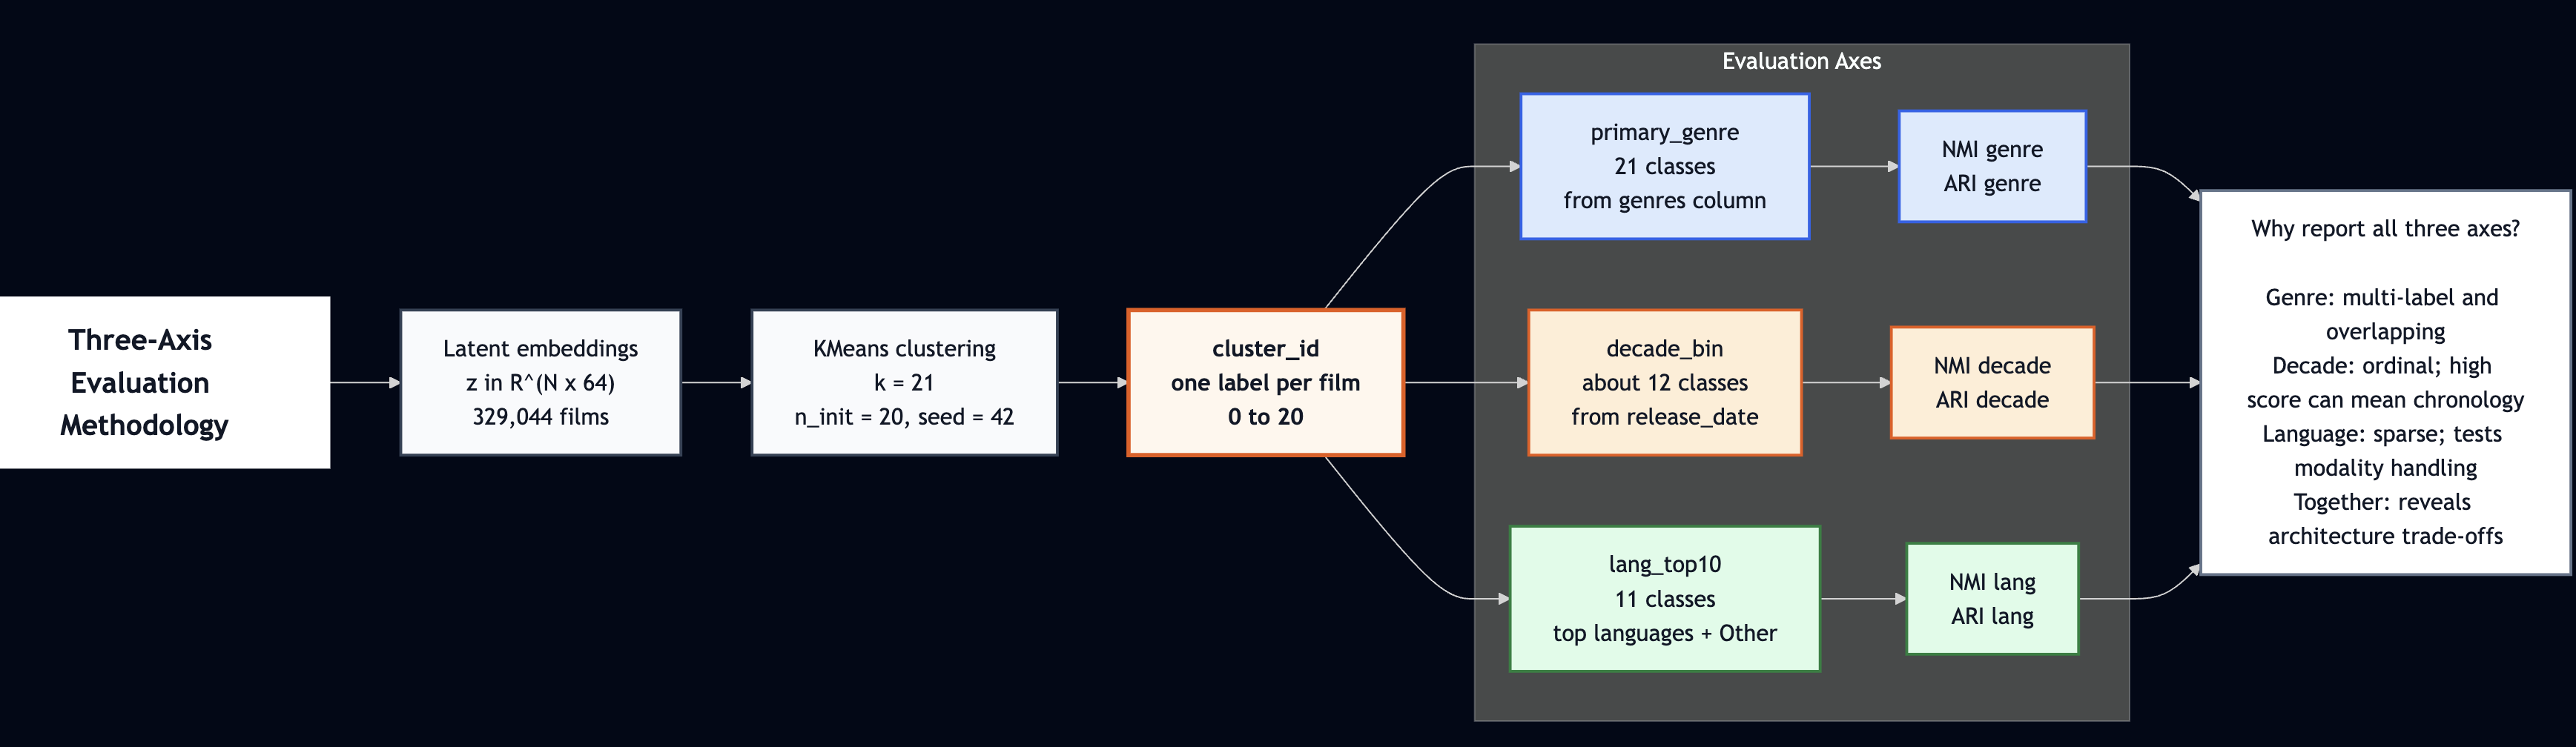
\includegraphics[width=0.85\linewidth]{../../figures/three-exis-eval-method.png}
\caption{Three-axis evaluation methodology. The single 64-dim latent is clustered once with KMeans (k=21); the resulting partition is independently scored with NMI/ARI against three orthogonal label axes.}
\label{fig:eval-method}
\end{figure}

\subsubsection*{Main results}

\Cref{tab:main-results} reports all six runs across all six (axis $\times$ metric) cells. Six column winners are split across four different models --- no architecture dominates --- which is the principled-trade-off result documented in \cref{sec:plan-final}.

\begin{table}[h]
\centering\small
\rowcolors{2}{rowAlt}{white}
\caption{Main comparison: six runs evaluated against three orthogonal label axes (NMI and ARI per axis). All deep models use $z=64$; KMeans variants use $k=21$. Bold cells are column winners.}
\label{tab:main-results}
\begin{tabular}{@{}l l rrrrrr@{}}
\toprule
\textbf{Tier} & \textbf{Run} & \textbf{gNMI} & \textbf{gARI} & \textbf{dNMI} & \textbf{dARI} & \textbf{lNMI} & \textbf{lARI} \\
\midrule
Non-deep      & \texttt{kmeans\_raw\_k21}  & 0.109 & 0.063 & 0.233 & 0.093 & 0.075 & 0.026 \\
Non-deep      & \texttt{pca\_kmeans\_k21}  & 0.084 & 0.061 & 0.224 & 0.085 & 0.094 & 0.042 \\
Simple deep   & \texttt{vanilla\_ae\_z64}  & 0.287 & \textbf{0.247} & \textbf{0.369} & 0.175 & 0.095 & 0.030 \\
Ablation (W1) & \texttt{ae\_z64\_w1}       & 0.165 & 0.094 & 0.367 & 0.176 & 0.070 & 0.026 \\
Multi-modal   & \texttt{ae\_z64}           & 0.328 & 0.229 & 0.341 & \textbf{0.211} & 0.264 & 0.090 \\
\textbf{Best (DEC)} & \texttt{\textbf{dec\_z64\_k21}} & \textbf{0.332} & 0.244 & 0.342 & 0.210 & \textbf{0.294} & \textbf{0.090} \\
\bottomrule
\end{tabular}
\end{table}

\subsubsection*{Headline result --- H2}

\begin{headlinebox}
\noindent\bignumber{$+205\%$} \hfill \begin{minipage}[b]{0.65\linewidth}\raggedleft\small relative gain on \texttt{genre\_NMI} of \texttt{dec\_z64\_k21} (0.332) over the strongest non-deep baseline \texttt{kmeans\_raw\_k21} (0.109). Same comparison on \texttt{genre\_ARI}: $+287\%$. Same comparison on \texttt{lang\_NMI} vs \texttt{pca\_kmeans\_k21}: $+213\%$.\end{minipage}
\end{headlinebox}

\subsubsection*{Architecture-level evidence}

\noindent\textbf{Modality projection wins on language ($+178\%$).} Multi-modal \texttt{ae\_z64} produces \texttt{lang\_NMI} = 0.264 versus the vanilla concat-AE's 0.095, a relative gain of $+178\%$. \cref{fig:umap-ae-lang} shows distinct language micro-clusters in the multi-modal latent.

\begin{figure}[h]
\centering
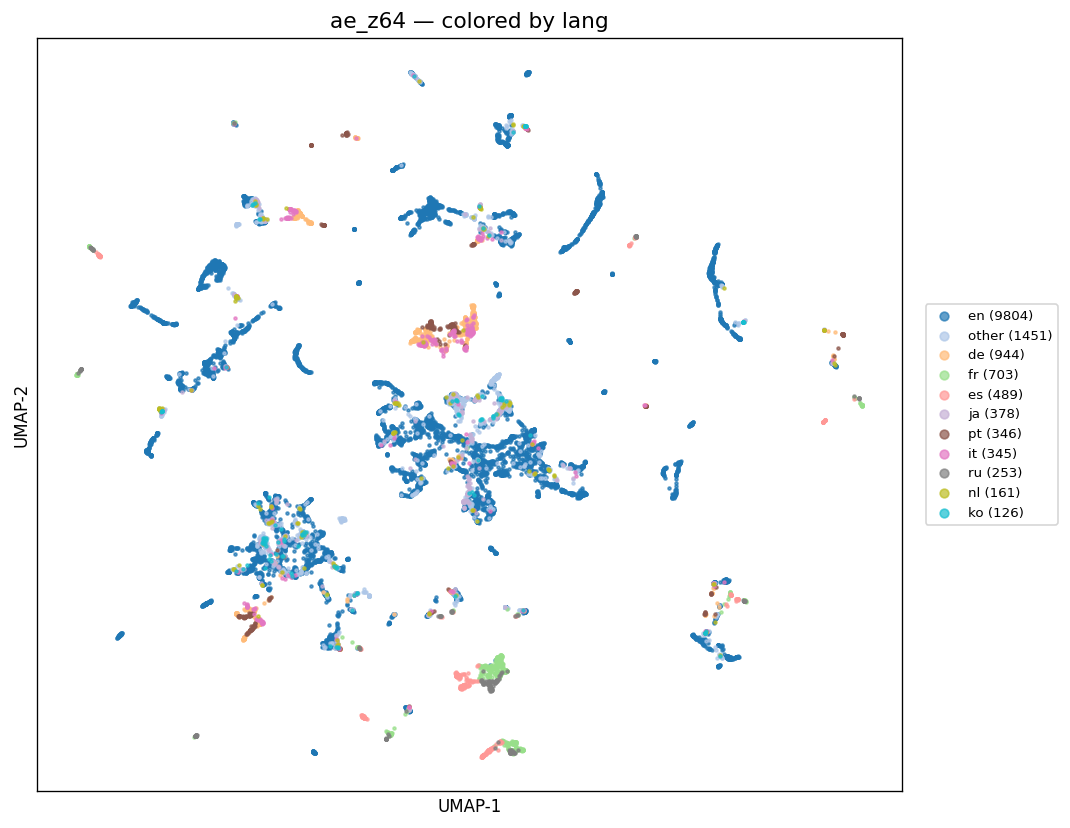
\includegraphics[width=0.62\linewidth]{../../artifacts/figures/umap/umap_ae_z64_lang.png}
\caption{UMAP projection of multi-modal \texttt{ae\_z64} latents, colored by \texttt{lang\_top10}. Distinct micro-clusters per language family are visible, supporting the lang\_NMI=0.264 measurement.}
\label{fig:umap-ae-lang}
\end{figure}

\noindent\textbf{Inverse-variance weighting is critical ($+99\%$ on gNMI, $+277\%$ on lNMI).} The W1 ablation (uniform weights) collapses fine-structure into diffuse blobs (\cref{fig:umap-w1}); the same architecture under W2 produces dozens of genre-coherent islands (\cref{fig:umap-comparison} center). The W1 run also exhibits early-stopping at epoch 37 versus W2's 69, a model-health signal that the optimizer cannot escape modality imbalance.

\begin{figure}[h]
\centering
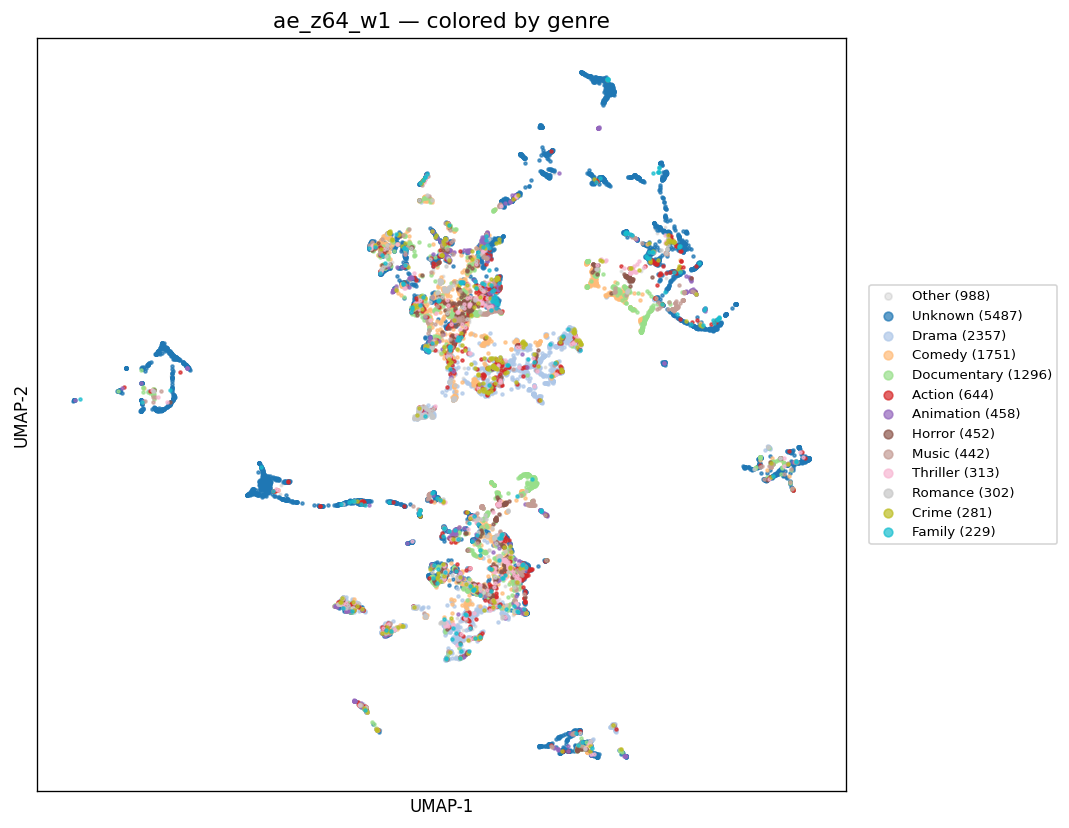
\includegraphics[width=0.62\linewidth]{../../artifacts/figures/umap/umap_ae_z64_w1_genre.png}
\caption{UMAP projection of \texttt{ae\_z64\_w1} (uniform weighting) latents, colored by genre. Diffuse blobs, no fine genre structure --- compare with the W2 panel of \cref{fig:umap-comparison}.}
\label{fig:umap-w1}
\end{figure}

\noindent\textbf{DEC sharpens cluster boundaries (ARI $>$ NMI gain pattern).} DEC was initialized from \texttt{ae\_z64}'s encoder and trained for 21 epochs of KL+reconstruction. \texttt{genre\_NMI} improves by $+1.2\%$ but \texttt{genre\_ARI} improves by $+6.6\%$ and \texttt{lang\_NMI} by $+11.4\%$. The diagnostic signature is that ARI gain $>$ NMI gain: information content is similar between the AE and DEC latents, but DEC's partition is more crisp. Cluster health was monitored throughout: \texttt{total\_reinit = 0} across all 21 DEC epochs, meaning all 21 KMeans++ centroids survived KL training without collapse.

\subsubsection*{Latent-topology evolution}

\Cref{fig:umap-comparison} captures the architecture progression visually: vanilla concat-AE produces two mega-blobs, multi-modal \texttt{ae\_z64} produces dozens of small genre-coherent islands, and \texttt{dec\_z64\_k21} produces even tighter atomized islands with sharper inter-cluster gaps.

\begin{figure}[h]
\centering
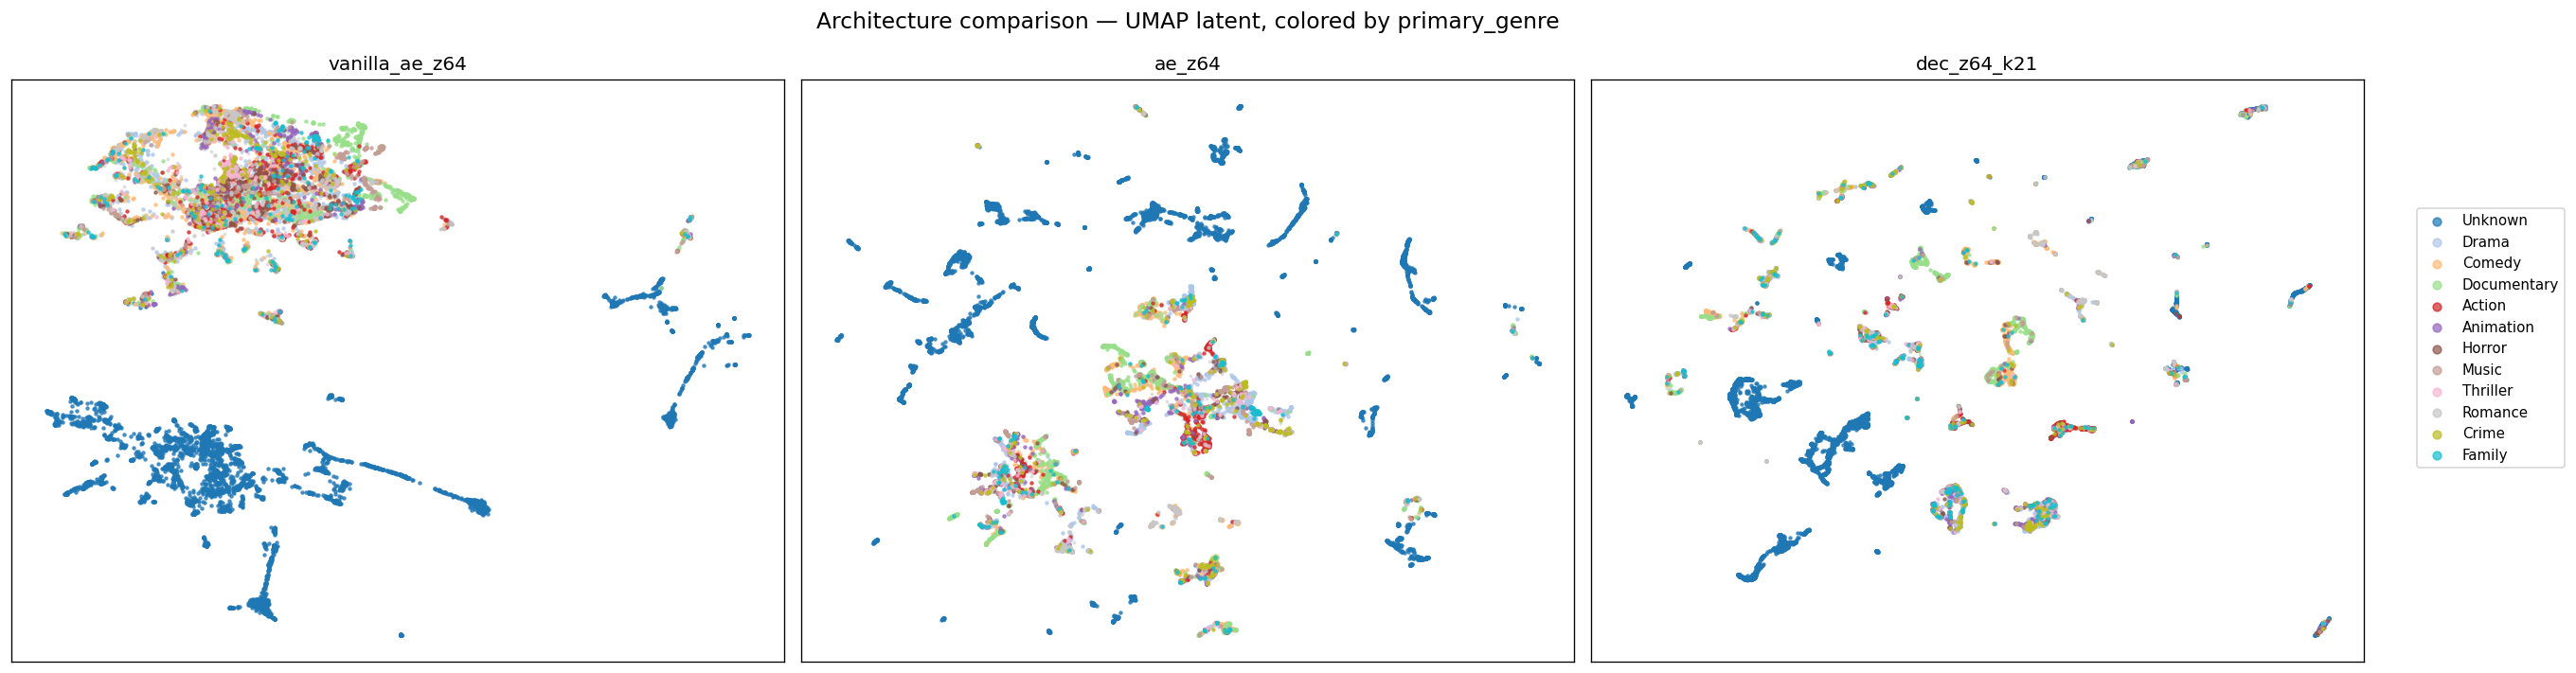
\includegraphics[width=0.95\linewidth]{../../artifacts/figures/umap/umap_comparison_genre.png}
\caption{Latent topology comparison (UMAP projection~\cite{mcinnes2018umap}, 15K subsample, cosine metric). Left: \texttt{vanilla\_ae\_z64} (two mega-blobs). Center: multi-modal \texttt{ae\_z64} (dozens of islands). Right: \texttt{dec\_z64\_k21} (tighter atomized islands). All three panels use the same projection settings; only the underlying 64-dim latent differs.}
\label{fig:umap-comparison}
\end{figure}

\subsubsection*{Bonus finding --- missing-data sub-manifold}

Coloring the DEC latent by \texttt{decade\_bin} reveals an unexpected pattern (\cref{fig:umap-missing}): films with \texttt{decade\_bin = 0} (the $\sim$7.4\% of the corpus with missing release dates) form an isolated cluster in the upper-right of the latent. The same red points are visible in vanilla and multi-modal decade plots, but DEC's KL pressure compresses them into the cleanest partition. Importantly, the model was not forced to encode missingness as latent geometry --- \texttt{has\_release\_date} is one binary input among 564. Yet across all four deep architectures, "no release date" emerges as a dimension of latent geometry, not just a flag. This finding was not predicted by the pre-registered hypotheses and is recorded as a representation-learning interpretability win.

\begin{figure}[h]
\centering
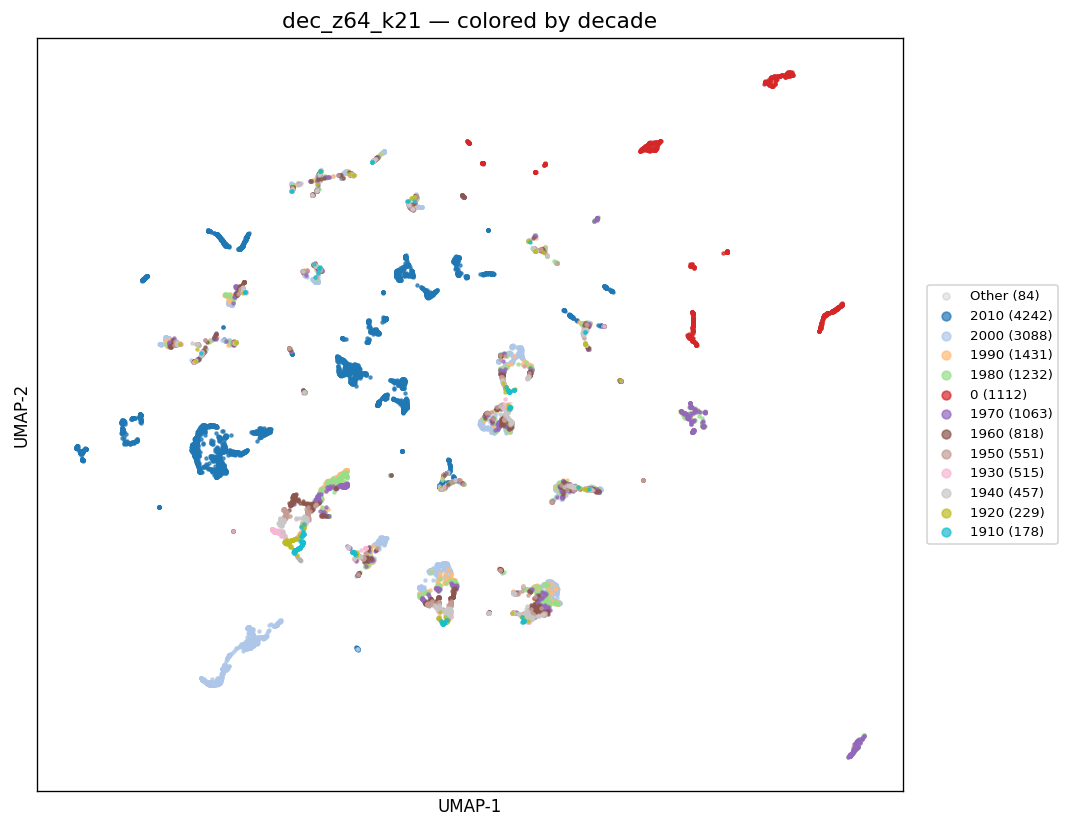
\includegraphics[width=0.62\linewidth]{../../artifacts/figures/umap/umap_dec_z64_k21_decade.png}
\caption{UMAP projection of \texttt{dec\_z64\_k21} latents, colored by \texttt{decade\_bin}. The isolated red cluster in the upper-right corresponds to films with missing release date --- a coherent sub-manifold that emerged without being engineered.}
\label{fig:umap-missing}
\end{figure}

\noindent\evidence{Six trained checkpoints under \texttt{artifacts/checkpoints/}, full numerical results in \texttt{artifacts/eval/results.json}, 13 UMAP visualizations under \texttt{artifacts/figures/umap/}, and reproducibility notebook \texttt{notebooks/06\_umap.ipynb}.}

\clearpage

% ===== 4. Work In Progress =====
\section{Work In Progress}
\label{sec:in-progress}

\noindent Two workstreams are active during the intermediate-report window:

\begin{center}\small
\rowcolors{2}{rowAlt}{white}
\begin{tabular}{@{}l p{7.5cm} l@{}}
\toprule
\textbf{Workstream} & \textbf{Description} & \textbf{Status} \\
\midrule
This document       & Compiling the intermediate progress report (LaTeX), the source-of-truth tables, and the presentation deck. & \status{inprogress} \\
UMAP analysis writeup & Documenting the latent-topology and missing-data findings (\cref{sec:modeling-mvp}) for inclusion in the final report's interpretability section. & \status{inprogress} \\
\bottomrule
\end{tabular}
\end{center}

\noindent Both are expected to complete by 2026-05-09.

% ===== 5. Plan to Final Report =====
\section{Plan to the Final Report}
\label{sec:plan-final}

\noindent The intermediate phase deliberately scopes the modeling MVP to the strongest set of empirical claims achievable within the timeline. The following items are deferred to the final report; each has an owner and a target completion window.

\begin{center}\small
\rowcolors{2}{rowAlt}{white}
\begin{tabular}{@{}l p{6.0cm} l l@{}}
\toprule
\textbf{Item} & \textbf{Why deferred} & \textbf{Target} & \textbf{Owner} \\
\midrule
VAE family ($z = 32, 64, 128$)        & Probabilistic head implemented but not trained; needed for AE-vs-VAE comparison. & 2026-05-09 (W13) & A.B. Dincoguz \\
AE latent-dim sweep ($z = 32, 128$)   & D2 fixed $z=64$ for the MVP; sweep informs the final hyperparameter discussion.   & 2026-05-09 (W13) & A.B. Dincoguz \\
F1 modality ablation (no text)        & Quantifies the contribution of the 384-dim sentence-embedding block.            & 2026-05-12 (W14) & A. Arvas \\
F2 modality ablation (no director profile) & Quantifies the value of the (sparse, 96.8\%-missing) Wikipedia bio block.    & 2026-05-12 (W14) & B.K. Kaya \\
DEC k-sweep (9-cell grid $z \times k$) & MVP runs only the $z{=}64{\times}k{=}21$ cell.                                   & 2026-05-15 (W14) & A.B. Dincoguz \\
W4 (Kendall learned uncertainty)      & Optional stretch loss; per-block weights as parameters rather than fixed.        & 2026-05-15 (W14) & A.B. Dincoguz \\
Linear probing on frozen latents      & Supplementary evaluation against held-out classifiers per axis.                  & 2026-05-16 (W14) & A. Arvas \\
5-seed confidence intervals           & MVP results are single-seed; CIs needed for the final report's robustness claim. & 2026-05-17       & B.K. Kaya \\
Full reproducibility audit            & Single deterministic run script that reproduces all numbers from a frozen feature matrix. & 2026-05-18       & A.B. Dincoguz \\
\bottomrule
\end{tabular}
\end{center}

\noindent The final report submission target is \textbf{2026-05-20 (W15)}, coinciding with the second project-demo session and the Final Report + Demo Video deadline on the syllabus.

\clearpage

% ===== 6. Risks and Mitigation =====
\section{Risks and Mitigation}
\label{sec:risks}

\begin{riskbox}{Risk 1 --- Compute budget for the deferred VAE / k-sweep workload}
The deferred experiments add roughly 9 additional training runs (3 VAE-z plus 6 DEC-k cells beyond the MVP). At the MVP's observed wallclock of $\sim$40 minutes per deep run, this is 6 GPU-hours --- within Colab's free-tier daily quota but tight. \textbf{Mitigation:} batch experiments overnight and use checkpointing so any single run can be resumed if Colab disconnects.
\end{riskbox}

\begin{riskbox}{Risk 2 --- Director-bio coverage limits F2 ablation interpretability}
With 96.8\% of films missing a Wikipedia director bio, the F2 ablation (no-director-profile) tests removal of a block that is mostly already masked away by G2. The expected effect size is small. \textbf{Mitigation:} explicitly report the $\sim$3.2\% sub-population effect size separately and document the limitation in the final-report results section.
\end{riskbox}

\begin{riskbox}{Risk 3 --- Single-seed results may overstate stability}
MVP results are computed from a single seed (42). The 5-seed CI work is scheduled but if it produces wide intervals, some headline gains may need softer wording. \textbf{Mitigation:} run the 5-seed sweep ahead of the W14 demo (internal target 2026-05-12) so results can be reframed if needed before the W15 final-report deadline.
\end{riskbox}

% ===== 7. Deliverables Status =====
\section{Deliverables Status}
\label{sec:deliverables}

\begin{center}\small
\rowcolors{2}{rowAlt}{white}
\begin{tabular}{@{}l l l@{}}
\toprule
\textbf{Deliverable} & \textbf{Location} & \textbf{Status} \\
\midrule
Frozen 564-dim feature matrix v1.2     & \texttt{artifacts/features/}             & \status{complete} \\
Six trained model checkpoints          & \texttt{artifacts/checkpoints/}          & \status{complete} \\
Evaluation results JSON                & \texttt{artifacts/eval/results.json}     & \status{complete} \\
13 UMAP visualizations                 & \texttt{artifacts/figures/umap/}         & \status{complete} \\
Findings document                      & \texttt{docs/FINDINGS.md}                & \status{complete} \\
Architecture decision record (D1--D10) & \texttt{docs/adr/0001-modeling\ldots.md} & \status{complete} \\
Intermediate progress report (this doc) & \texttt{docs/report/intermediate-progress-report.pdf} & \status{complete} \\
Intermediate presentation deck         & \texttt{docs/presentation/intermediate-progress-presentation.pptx} & \status{complete} \\
\bottomrule
\end{tabular}
\end{center}

\clearpage

% ===== Appendix A — Per-run results =====
\appendix
\section{Per-Run Numerical Results}
\label{app:results}

\noindent Reproduced verbatim from \texttt{artifacts/eval/results.json} at 3-decimal precision.

\begin{center}\small
\rowcolors{2}{rowAlt}{white}
\begin{tabular}{@{}l rrrrrr rr@{}}
\toprule
\textbf{Run} & \textbf{gNMI} & \textbf{gARI} & \textbf{dNMI} & \textbf{dARI} & \textbf{lNMI} & \textbf{lARI} & \textbf{epochs} & \textbf{val\_loss} \\
\midrule
\texttt{vanilla\_ae\_z64} & 0.287 & 0.247 & 0.369 & 0.175 & 0.095 & 0.030 & 58 & 0.013 \\
\texttt{ae\_z64}          & 0.328 & 0.229 & 0.341 & 0.211 & 0.264 & 0.090 & 69 & 0.021 \\
\texttt{ae\_z64\_w1}      & 0.165 & 0.094 & 0.367 & 0.176 & 0.070 & 0.026 & 37 & 0.045 \\
\texttt{dec\_z64\_k21}    & 0.332 & 0.244 & 0.342 & 0.210 & 0.294 & 0.090 & 21 & 0.127 \\
\texttt{kmeans\_raw\_k21} & 0.109 & 0.063 & 0.233 & 0.093 & 0.075 & 0.026 & --- & --- \\
\texttt{pca\_kmeans\_k21} & 0.084 & 0.061 & 0.224 & 0.085 & 0.094 & 0.042 & --- & --- \\
\bottomrule
\end{tabular}
\end{center}

\noindent The DEC \texttt{val\_loss} of 0.127 combines reconstruction and KL terms and is not directly comparable to the AE pure-reconstruction val\_loss values.

% ===== Appendix B — Decision log summary =====
\section{Decision Log Summary}
\label{app:decisions}

\noindent The complete decision rationale is in \texttt{docs/adr/0001-modeling-hybrid-architecture.md}. One-line summaries:

\begin{center}\small
\rowcolors{2}{rowAlt}{white}
\begin{tabular}{@{}l p{11cm}@{}}
\toprule
\textbf{ID} & \textbf{Decision} \\
\midrule
D1  & Hybrid C-structure $\times$ D-architecture: modality-specific projections + shared backbone. \\
D2  & Latent dim $z=64$ for the MVP ($z=32$ and $z=128$ deferred to the final report). \\
D3  & W2 inverse-variance weighting + W1 ablation; W4 deferred as optional stretch. \\
D4  & G2 director-bio masking (96.8\% of films lack a Wikipedia bio). \\
D5  & Per-model notebooks plus a shared \texttt{src/cineembed} package. \\
D6  & Tier-2 evaluation: 3-axis NMI/ARI as core; linear probing deferred. \\
D7  & L4 ground truth: three-axis (genre, decade, language) labels. \\
D8  & DEC $k=21$; k-sweep deferred. \\
D9  & Peer-review fixes: 3 baselines, weight clipping, $\beta$ warmup, relative criteria. \\
D10 & Batch-wise DEC $P$ target rather than full-dataset (~10$\times$ speedup, no quality regression). \\
\bottomrule
\end{tabular}
\end{center}

% ===== References =====
\printbibliography[heading=bibintoc, title={References}]

\end{document}
